%Version 2.1 April 2023
% See section 11 of the User Manual for version history
%
%%%%%%%%%%%%%%%%%%%%%%%%%%%%%%%%%%%%%%%%%%%%%%%%%%%%%%%%%%%%%%%%%%%%%%
%%                                                                 %%
%% Please do not use \input{...} to include other tex files.       %%
%% Submit your LaTeX manuscript as one .tex document.              %%
%%                                                                 %%
%% All additional figures and files should be attached             %%
%% separately and not embedded in the \TeX\ document itself.       %%
%%                                                                 %%
%%%%%%%%%%%%%%%%%%%%%%%%%%%%%%%%%%%%%%%%%%%%%%%%%%%%%%%%%%%%%%%%%%%%%

%%\documentclass[referee,sn-basic]{sn-jnl}% referee option is meant for double line spacing

%%=======================================================%%
%% to print line numbers in the margin use lineno option %%
%%=======================================================%%

%%\documentclass[lineno,sn-basic]{sn-jnl}% Basic Springer Nature Reference Style/Chemistry Reference Style

%%======================================================%%
%% to compile with pdflatex/xelatex use pdflatex option %%
%%======================================================%%

%%\documentclass[pdflatex,sn-basic]{sn-jnl}% Basic Springer Nature Reference Style/Chemistry Reference Style


%%Note: the following reference styles support Namedate and Numbered referencing. By default the style follows the most common style. To switch between the options you can add or remove “Numbered” in the optional parenthesis. 
%%The option is available for: sn-basic.bst, sn-vancouver.bst, sn-chicago.bst, sn-mathphys.bst. %  
 
%%\documentclass[sn-nature]{sn-jnl}% Style for submissions to Nature Portfolio journals
%%\documentclass[sn-basic]{sn-jnl}% Basic Springer Nature Reference Style/Chemistry Reference Style
\documentclass[sn-mathphys, Numbered]{sn-jnl}% Math and Physical Sciences Reference Style
%%\documentclass[sn-aps]{sn-jnl}% American Physical Society (APS) Reference Style
%%\documentclass[sn-vancouver,Numbered]{sn-jnl}% Vancouver Reference Style
%%\documentclass[sn-apa]{sn-jnl}% APA Reference Style 
%%\documentclass[sn-chicago]{sn-jnl}% Chicago-based Humanities Reference Style
%%\documentclass[default]{sn-jnl}% Default
%%\documentclass[default,iicol]{sn-jnl}% Default with double column layout

%%%% Standard Packages
%%<additional latex packages if required can be included here>

\usepackage{graphicx}%
\graphicspath{ {./Figures/} }
\usepackage{multirow}%
\usepackage{amsmath,amssymb,amsfonts}%
\usepackage{amsthm}%
\usepackage{mathrsfs}%
\usepackage[title]{appendix}%
\usepackage{xcolor}%
\usepackage{textcomp}%
\usepackage{manyfoot}%
\usepackage{booktabs}%
\usepackage{algorithm}%
\usepackage{algorithmicx}%
\usepackage{algpseudocode}%
\usepackage{listings}%
\usepackage[
style=apa
]{biblatex}%
\addbibresource{myref.bib}
\addbibresource{references.bib}
\addbibresource{rawrefs.bib}

\RequirePackage{enumitem} % For reducing bullet list item separation
\newcommand\posscite[1]{\citeauthor{#1}'s \parencite*{#1}}
%%%%

%%%%%=============================================================================%%%%
%%%%  Remarks: This template is provided to aid authors with the preparation
%%%%  of original research articles intended for submission to journals published 
%%%%  by Springer Nature. The guidance has been prepared in partnership with 
%%%%  production teams to conform to Springer Nature technical requirements. 
%%%%  Editorial and presentation requirements differ among journal portfolios and 
%%%%  research disciplines. You may find sections in this template are irrelevant 
%%%%  to your work and are empowered to omit any such section if allowed by the 
%%%%  journal you intend to submit to. The submission guidelines and policies 
%%%%  of the journal take precedence. A detailed User Manual is available in the 
%%%%  template package for technical guidance.
%%%%%=============================================================================%%%%

%\jyear{2023}%

%% as per the requirement new theorem styles can be included as shown below
\theoremstyle{thmstyleone}%
\newtheorem{theorem}{Theorem}%  meant for continuous numbers
%%\newtheorem{theorem}{Theorem}[section]% meant for sectionwise numbers
%% optional argument [theorem] produces theorem numbering sequence instead of independent numbers for Proposition
\newtheorem{proposition}[theorem]{Proposition}% 
%%\newtheorem{proposition}{Proposition}% to get separate numbers for theorem and proposition etc.

\theoremstyle{thmstyletwo}%
\newtheorem{example}{Example}%
\newtheorem{remark}{Remark}%

\theoremstyle{thmstylethree}%
\newtheorem{definition}{Definition}%

\raggedbottom
%%\unnumbered% uncomment this for unnumbered level heads

\begin{document}

\title[Article Title]{Exploring the Use of GPT-4 when Generating Personalized Case Scenarios for Higher Education.}

%%=============================================================%%
%% Prefix	-> \pfx{Dr}
%% GivenName	-> \fnm{Joergen W.}
%% Particle	-> \spfx{van der} -> surname prefix
%% FamilyName	-> \sur{Ploeg}
%% Suffix	-> \sfx{IV}
%% NatureName	-> \tanm{Poet Laureate} -> Title after name
%% Degrees	-> \dgr{MSc, PhD}
%% \author*[1,2]{\pfx{Dr} \fnm{Joergen W.} \spfx{van der} \sur{Ploeg} \sfx{IV} \tanm{Poet Laureate} 
%%                 \dgr{MSc, PhD}}\email{iauthor@gmail.com}
%%=============================================================%%

\author*[1]{\fnm{Pablo} \sur{Flores}}\email{pablo.flores@helsinki.fi}

\author[1]{\fnm{Guang} \sur{Rong}}\email{guang.rong@helsinki.fi }

\author[1,2]{\fnm{Benjamin Ultan} \sur{Cowley}}\email{ben.cowley@helsinki.fi}


\affil*[1]{\orgdiv{Faculty of Educational Sciences}, \orgname{University of Helsinki}, \orgaddress{\street{Siltavuorenperger 5}, \city{Helsinki}, \postcode{00014 },  \country{Finland}}}
\affil*[2]{\orgdiv{Cognitive Science, Faculty of Arts}, \orgname{University of Helsinki}}


%%==================================%%
%% sample for unstructured abstract %%
%%==================================%%

\abstract{In the fast evolving landscape of Artificial Intelligence in Education (AIEd), Large Language Models (LLMs) like GPT-4 have emerged as powerful and versatile tools capable of adapting for a wide set of natural language tasks. LLMs can interact as though they understand language, yet they remain algorithms and can be used as such. This study explores a novel guided interaction design for modeling users' information foraging behavior when navigating GPT-generated content and the role of Computational Thinking skills in shaping such behavior. Conducted with nine educational researchers in a doctoral-level AIEd course, our research used editable prompt templates and keywords to structure the prompt crafting process . We modeled and analyzed participants' behaviors in terms of \textit{exploration} (to generate and explore various information landscapes) and \textit{exploitation} (to delve deeper in a specific landscape). Our data, including responses from the Computational Thinking Scale, suggests that Algorithmic Thinking and Creativity might encourage \textit{exploitation} behavior, leaning more on AI-generated information rather than pre-defined design elements. Furthermore, including participants' interests into the interaction design seems to foster a shared conceptual space in prompt construction. This approach encouraged the use and combination of diverse interests for content creation, as opposed to relying solely on individuals' interests. Our findings also suggest that \textit{exploitation} prompts are predominantly driven by GPT-generated content. While this seems to add value to AI-generated content, it raises concerns about potential overreliance, specially in educational settings.}

%%================================%%
%% Sample for structured abstract %%
%%================================%%

\keywords{ChatGPT 4, Large Language Models, Higher Education, Human-LLM interaction, Exploration, Exploitation, Computational Thinking}

%%\pacs[JEL Classification]{D8, H51}

%%\pacs[MSC Classification]{35A01, 65L10, 65L12, 65L20, 65L70}

\maketitle

\section{Introduction}

% Digital tech in education - reshaping the landscape.
Upon every technological breakthrough, the educational domain reconsiders its methods and strategies. During the recent decades, the rise of digital technologies has reshaped the educational landscape. Evidence from the past 40 years of studies on educational technologies consistently indicates positive benefits from its integration in programming courses or through innovative approaches \parencite{higgins_impact_2012}.  

However, while digital technologies might spark motivation and engagement in young students, its mere adoption does not ensure favorable outcomes.  To fully embrace their potential, a deliberate pedagogical approach is essential, especially when transitioning from traditional to modern educational approaches \parencite{parker_authentic_2020,khaddage_bridging_2021} . 

% AIEd - Extensive, but limited, integration of recent new technologies
As part of the larger digital transformation, Artificial-Intelligence (AI)-based systems have emerged as important players in the educational domain. These systems have found extensive use in administration, instruction, and learning \parencite{chen_application_2020}, accompanied by a growing body of research around AI in Education (AIEd), a distinct sub-field of digital learning research \parencite{niemi_ai_2023}.  But despite the wide range of potential applications of AI-based systems, they have been mostly implemented to facilitate, or automate, mainstream learning approaches. While useful, this approach sidelines teachers agency, experience, and creativity to integrate such technologies into their unique practices and pedagogical designs. \parencite{holmes_artificial_2023}

%  Dominant trend of STEM design in AIEd
A dominant trend has been that AIEd implementations are predominantly designed by technical teams or departments, such as those focused in Science, Technology, Engineering, and Math (STEM), leading to a notable under-representation of educational or psychological perspectives in AIEd research \parencite{holmes_state_2022, zawacki-richter_systematic_2019}. Among the probable causes of this we can highlight the lack of technical expertise, among others, which is a big barrier for educational adoption of technologies \parencite{reid_categories_2014}. However, as with other digital technologies, AI systems are evolving to become more accessible by reducing their technical entry barriers, both for casual use and for the design of new applications.

%  LLMs - Recent developments offer incredible opportunities
One such evolution is Large Language Models (LLMs) such as OpenAI's Generative Pre-trained Transformer (GPT) model. LLMs have significantly evolved into systems capable of performing various natural language tasks \parencite{brown_language_2020}. Interestingly, they have shown emergent features as they are able to perform tasks that were not originally part, or expected, of the design \parencite{wei_emergent_2022}. For example, GPT-3 could adapt to new tasks using an approach known as \textit{In-context learning}---relying on natural language descriptions of the task---an ability that its predecessor struggled to perform consistently \parencite{brown_language_2020, wei_emergent_2022}. This adaptation for different tasks, without requiring extensive re-design of the model's architecture, combined with their potential to serve as building blocks for task-specific AI tools, has led to some researchers to classify them as foundational models \parencite{eloundou_gpts_2023, bommasani_opportunities_2022}.  Furthermore, last iteration (GPT-4) brought a significant increase in performance across every measured metric \parencite{openai2023gpt4}.
These capabilities present wide opportunities in both design and application. Given that state-of-the-art models do not require advanced technical programming skills, professionals from different domains can now tailor customized tools that align closely with their contexts, needs, and specialized approaches \parencite{cain_gpteammate_2023}. Building on this accessibility, OpenAI has recently announced the "GPT builder", which enables users to tailor specific web-based GPT applications for private or shared use \parencite{openaidevshowcase, openai_introducing_2023}. Altogether, a new generation of commercial, public, and private LLM-based AI applications is on the horizon, with many speculated to be significant in shaping the near to mid-term future \parencite{bommasani_opportunities_2022, bubeck_sparks_2023}. 

% P4 - ChatGPT - Free and widespread chatbot application of GPT-4. Conversational dynamic
Due to its versatility and accessibility, OpenAI's "ChatGPT" has become the fastest-growing application in history since its launch on late 2022 \parencite{milmo_chatgpt_2023}. As a conversational chatbot, it uses natural language processing to understand and generate human-like text in a dialectical fashion. By providing certain input (prompts) ChatGPT can answer different kinds of questions. Additionally, by using advanced prompting methods users can improve its performance in a wide range of tasks \parencite{wei_chain--thought_2023,fernando_promptbreeder_2023}. Potential educational uses involve teaching preparation (generation of course materials, providing suggestions); Assessment (generation of exercises or case scenarios, providing feedback); Learning support (answering questions, summarising information) among others \parencite{lo_what_2023,montenegro-rueda_impact_2023}.  However, educational research remains sparse and focuses predominantly in theoretically exploring its potential and limitations \parencite{qadir_engineering_2022,cain_gpteammate_2023}, and assessing its performance on traditional assessment methods \parencite{nisar_is_2023}. Due to its novelty, a gap in exploratory empirical studies is evident.

We focused our study on exploring how modes of cognition govern the interaction between doctoral researchers and GPT-4 for the creation of personalized course materials in a higher education doctoral course. Studies in web searching tasks have shown that information foraging agents are constantly balancing between \textit{exploration} and \textit{exploitation} types of decision making, visible in their task behavior and actions \parencite{pirolli_information_1999, pirolli_rational_2005, pirolli_information_2007}.  By drawing from these theoretical contributions of Information Foraging Theory in understanding Human-Computer Interactions, we designed a controlled interaction to analyze humans' decision-making when foraging within AI generated informational landscapes. Additionally, we explore the influence of Computational Thinking skills in modulating participants' foraging behavior.



\subsection*{Approach}\label{Approach}  


% The context higher education course regarding AI in education
The study was conducted in an on-campus doctoral course titled “Basics of AI in education”, which aimed at exploring historical and contemporary AIEd developments. It covered an overview of the historical technical evolution of AIEd systems, examination of current popular systems, like performance predictors, AI-tutors and LLMs, a review of the intersection between AI and cognitive sciences, as well as a discussion of emerging ethical concerns and regulatory developments. 

% Purpose of the course - Speculative assigments - flexible topics
The course assignments led students to explore hypothetical scenarios about AI implementations in education. For this purpose the students were asked to individually design a study, and write a reflective essay about a specific chosen scenario. Consequently, the course topics were broad and suggestive, not focused on any pre-defined scenario, giving the students freedom to choose a scenario of their own interest. 
Complementing the course contents with a practical experience, we guided the students to interactively generate their hypothetical scenarios with the support of AI. 


To facilitate this, we designed a guided interaction to co-create personalized hypothetical scenarios through GPT-4, which involved pre-defined \textit{prompt templates} and a \textit{set of keywords} to construct scenario generation prompts. Our design addressed three main objectives:

% Study/design purpose - To examine the behavioral aspects of students-GPT interactions
First, to standardize the interaction across students with diverse levels of experience with ChatGPT. Due to its novelty, we had to guide students without experience in interacting with ChatGPT. By providing clear guidelines and a set of actions to choose from, outlined by prompt templates, we expected that students lacking prior experience could complete their co-creation task without major technical challenges.
Second, to enable a systematic and reproducible examination of interactions with ChatGPT by establishing a controlled interaction protocol. The design not only standardizes how students interact with ChatGPT, but it can be tailored to capture specific elements according to our research interests, particularly the behavioral dimensions of students interaction.
% Information Foraging

Third, to facilitate behavioral modes from Information Foraging Theory. Given that ChatGPT has contextual memory of the conversation, it enables users not only to generate scenarios but also to coherently delve deeper by prompting for additional details, thus enriching the scenario with more information. This dynamic closely mirrors two core aspects of Information Foraging Theory: \textit{Exploration}, where new information landscapes are searched (generating scenarios), and \textit{Exploitation}, where agents decide to utilize a landscape to its fullest potential (further elaborating an interesting scenario) \parencite{todd_foraging_2020,hills_exploration_2015,cohen_should_2007}. Therefore we shape our prompt design around these distinct foraging actions, conceptualizing the interactions as a a decision-making process within an information foraging task. 

% Computational Thinking
Finally, we examined the role of Computational Thinking Skills in modulating students' interactions with ChatGPT. In a seminal contribution, Wing \parencite*{wing_computational_2006} underscored the importance of Computational Thinking skills, which enables people to solve tasks in a similar way that computer algorithms work and are beneficial across most professional domains. Since then, Computational Thinking Skills have grown into a cornerstone of research in digital education and different researchers argue that they correlate with more confident and efficient use of digital technologies \parencite{cansu_overview_2019,grover_computational_2013, shute_demystifying_2017}. Regarding the influence of Computational Thinking over Human-AI Interactions, Celik \parencite*{celik_exploring_2023} explored the determinants of AI literacy, which encompass the knowledge for using, recognizing and evaluating AI-based tools, and reported a significant correlation with Computational Thinking Skills.
Furthermore, Yilmaz \& Karaoglan \parencite*{yilmaz_effect_2023} found, through a controlled experiment, that allowing the use of ChatGPT in a programming course improved students' CTS scores.

Building on these contributions, we aim to delve deeper into the practical manifestations of such association. We pose the following research questions to investigate whether the unique nature of LLMs, distinct from other AI systems, might reveal new insights into Computational Thinking Skills within the evolving landscape of education. 
\begin{enumerate}[itemsep=.5em,leftmargin=.5in,label=\textbf{RQ\arabic*.}]
    \item How do students interact with ChatGPT-4 in terms of Exploration-Exploitation decision-making?
    \item How are students' Computational Thinking skills reflected in their interactions with GPT-4? 
\end{enumerate}



\section{Methods}\label{Methods}

This section describes our participants, the interaction design, and the measurements used, including the coding of interactions, and the Computational Thinking Scale. The study was carried out in accordance with the Declaration of Helsinki, with the ethical approval of the Research Ethics Committee in the Humanities and Social and Behavioural Sciences, University of Helsinki (27/2022). Informed consent was obtained from all participants.

\subsection*{Participants}

We conducted this study within an international doctoral course called "Basics on Artificial Intelligence in Educational Sciences" at the University of Helsinki. Initially, 16 students registered to the course, but only 12 completed it. We invited these students to join the study and 10 agreed to participate. All participants, but one, completed the scenario generation task resulting in a sample size of n = 9.

Participants ranged in age from 30 to 40 (mean = 32.8), with near equal gender distribution (5 females). Six of them were Finnish and the rest a combination of Chinese and Koreans, they all had fluent English skills. They specialized in different educational fields of research, such as Early Childhood Education, Educational Psychology, Science Education, and Higher Education. As the course was optional, we assume that all participants had previous interests towards AI applications in education, either for personal or research motivations. Five of them reported previous experiences in using ChatGPT for work, research or personal experiments. The other four reported no previous experience with ChatGPT, or similar applications. 


\subsection*{Guided Interaction Design}\label{Interaction design}

At the first class, we presented the main author to the students and the purpose of studying the development of the course; however, they were naive to the study's specific aims.
Our design consists of six modifiable \textit{prompt templates}, divided in two types; a \textit{set of keyword cards}, made of individual cards with relevant concepts gathered from participants' personal interests; and an \textit{interaction protocol}, outlining the interaction process. With these, participants crafted a diversity of prompts tailored to their interests, which were used to create and elaborate their hypothetical scenarios in ChatGPT. The interaction diagram in Figure \ref{fig:Interaction Diagram} provides a visual representation of this process.

\subsubsection*{\textit{Prompt Templates and Set of Keywords}}

Following the information foraging theoretical approach described above, we created the\textit{ prompt templates} to facilitate two main categories of action (see Table \ref{tab:prompt types}).

Firstly, we created three different \textit{Exploration prompts} aimed at creating unique scenarios. Their nature was defined by their start ("Describe to me a scenario..." and "Predict a future scenario...") and they allowed for the combination of a maximum of 6 keywords, which granted sufficient conceptual context for our co-creation aims. They provided the starting point to create and explore different scenarios and informational landscapes.

Secondly, we created three \textit{Exploitation prompts} to further elaborate already generated scenarios. They prompted for more information about the specified scenario, focusing in one, or two, keywords of interest. Therefore, they enabled the exploitation of an interesting scenario for more information.

This distinction between the two types of \textit{prompt templates} facilitates our analysis by enabling us to clearly categorize their use within the interaction as either \textit{exploration} or \textit{exploitation} actions.

To construct the \textit{set of keywords}, we envisioned seven categories that generally described AI-influenced educational scenarios (see Table \ref{tab:set of keywords}). So that participants' personal interests drove the interaction, these categories were populated based on an initial course assignment in which participants were asked to introduce themselves and their interests in relation to the aforementioned categories. This followed from \posscite{niemi_artificial_2023} concept of a socially-shared virtual environment that allows users to explore their own representation. Taking into account their reported interests fostered a student-driven approach to enhance the relevance and boost engagement of the participants with the task. 
As a result, we created a set of 86 keywords distributed unevenly across the different categories. This meant the conceptual context of every generated scenario was shaped by the participants' choices.

During the interaction, we allowed the participants to use keywords provided by ChatGPT. After observing its answers to the prompts, where ChatGPT generally offered bullet points to describe the main aspects of the generated scenario, participants could use point headers as keywords. These \textit{GPT's keywords} enabled more flexibility and precision, particularly if participants were prone to exploit an interesting scenario based on its specific conceptual information, which would not be necessarily present in the \textit{keywords set}. This added another interesting layer of theoretical depth, as we could observe how the \textit{Exploration} and \textit{Exploitation} of information acted with both human-generated concepts and AI-generated concepts.

Both the \textit{prompt templates} and the \textit{keywords} were printed and laminated. The \textit{prompt templates} consisted of a fixed text written in black representing unchangeable elements, along with colored spaces. These colored spaces corresponded to the different categories where participants could select and the \textit{set of keywords.} The keywords were represented as a series of color-coded cards, each card corresponding to an individual keyword and colored by category, to enable a more intuitive understanding of the interaction design.


\begin{table}
    \centering \caption{Prompt types examples}
    \begin{tabular}{c|c}
         Prompt type& Example\\
         \hline
         Exploration& Describe to me a scenario where we can see the [effect] for [actors]/[ed. process]\\
 & when using [AI tools] in a [environment] + [subject] + [activity]\\
         Exploitation& Tell me more about this scenario but put more emphasis on [element of interest]\\
         \hline
    \end{tabular}
    \label{tab:prompt types}
\end{table}


\begin{table}
    \centering \caption{Set of keywords' categories and examples.}
    \begin{tabular}{c|c|c|c|c|c|c|l}
         Category&  Effect&  Actors&  AI tools&  Ed. process&  Environment& Subject&Activity\\
         \hline
         \textit{Example}&  \textit{Assist}&  \textit{Teachers}&  \textit{GPT}&  \textit{Learning}&  \textit{School}&  \textit{Biology}&\textit{Lecture}\\
    \end{tabular}
    \label{tab:set of keywords}
\end{table}


To facilitate the interaction process, we designed an \textit{interaction protocol} to guide the use of the \textit{prompt templates} with the \textit{set of keywords}. This protocol guided the process, standardized the first author's role, and constrained his influence over the participants' decision-making process. This approach ensured sufficient agency for participants to drive the interaction, while maintaining a helpful guidance throughout the interaction.

\subsubsection*{\textit{Interaction Protocol}}

We scheduled individual sessions with each student for the task. The first author facilitated the sessions, guiding the participants over the co-creation process according to the following interaction protocol:
    \begin{itemize}

        \item  Prompt templates were displayed on a table along with the keywords cards, face down in 5 rows, divided by the coloured categories.
        \item Participants were briefed on the aim of the task---creating an interesting scenario for their assignments---and introduced to the use of prompt templates and keywords, including an example to illustrate their application. Usage information was reminded during the interaction to ensure effective performance with the task.
        \item When the aim and rules were clear, participants began by uncovering the first row of keywords, selecting a template and keywords of interest to craft a prompt. We then input the prompt to ChatGPT, read the generated text and participants chose their next option: to generate (\textit{explore}) new scenarios, further elaborate (\textit{exploit}) the current one, view more of the guide's keywords, or ending the task by choosing the scenario for their course assignment. We also highlighted the option of including GPT's keywords to explore or exploit scenarios.
        \item Once the participant decided that a scenario was interesting enough for them to end the task, we provided them with the full transcript of the conversation for the selected scenario.
    \end{itemize}

\begin{figure}
    \centering
    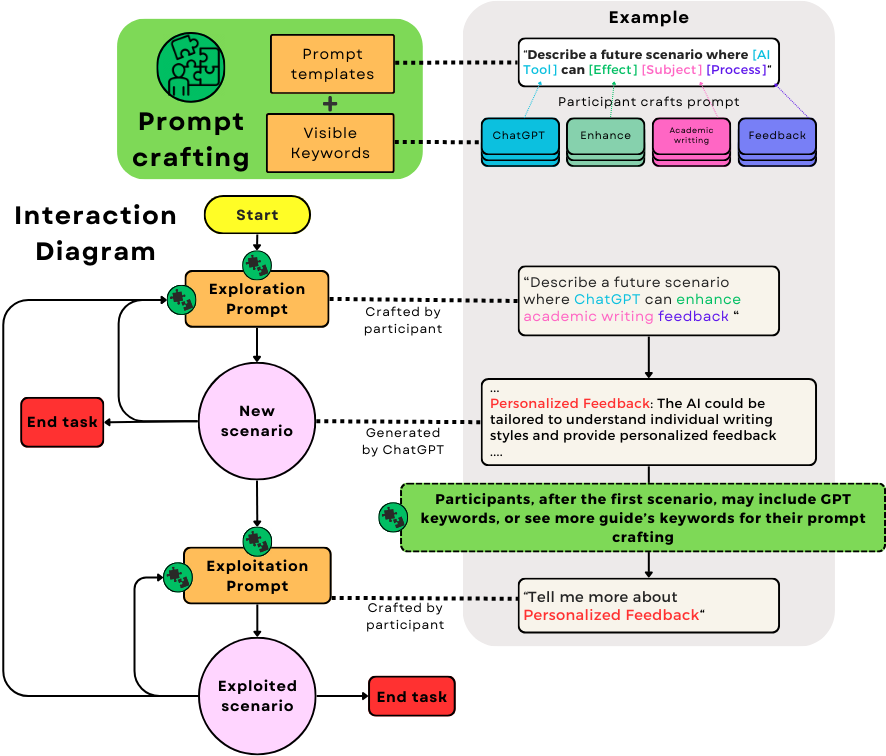
\includegraphics[width=1\linewidth]{Interaction diagram (5).png}
    \caption{Interaction Diagram. Participants craft their prompts by selecting a prompt templates and keywords of interest. The process initiates with an \textit{Exploration} prompt, to generate a hypothetical assignment scenarios. Subsequently, participants can select new templates and keywords, and craft prompts to \textit{explore} new scenarios, \textit{exploit} interesting scenarios, or end the task by choosing a scenario that is interesting for them. After viewing the first scenario, participants may view additional guide keywords or include GPT's keywords into their prompt crafting. Note: The examples provided are simplified; actual prompts and ChatGPT's responses are more detailed.}
    \label{fig:Interaction Diagram}
\end{figure}

\subsection*{Computational Thinking Scale}

To examine the role of Computational Thinking within our interaction process, and following Celik's previous study on AI literacy \parencite*{celik_exploring_2023}, we chose to employ the same instrument, the Computational Thinking Scale (CTS) survey.

Developed by Korkmaz et al. \parencite*{korkmaz_validity_2017}, CTS is a self-report scale based on the framework provided by the Computer Science Teachers Association (CSTA) with the International Society for Technology in Education (ISTE) \parencite*{csta_iste_operational_2015, iste_computational_2011}, and the Computational Thinking Leadership Toolkit \parencite{iste_ct_2015}. They define computational thinking as the result of 5 intertwined skills, Creativity, Algorithmic Thinking, Cooperativity, Critical Thinking, and Problem Solving. Consequently, the scale consists of 29 items divided in the corresponding 5 sub-factors. Based on a five-point Likert-type rating structure and after reversing the sub-factor of problem solving, higher scores indicate a greater development of computational thinking skills.

Additionally, because the scale was developed in computer sciences learning environments, we adapted three items' grammar and semantics, and adapted mathematically specific terms to be more general. The Cronbach's Alpha coefficients were recalculated and found to be 0.63 for creativity, 0.84 for algorithmic thinking, 0.9 for cooperativity, 0.95 for critical thinking, and 0.7 for problem solving. The coefficient for all items was 0.65.


\subsection*{Data Analysis}

We coded the behavioral data from the interactions using ATLAS.ti 23. A frequency-based data set was constructed based on the interactions' logs provided by ChatGPT. Additionally, we tracked the co-occurrence of coded variables. The frequency-based dataset encompassed 8 variables, which described the user choices derived from the prompt templates, keywords, and students' reported interests. (see Table \ref{tab:interaction variables}). 


\begin{table} \caption{Behavioral variables describing participants' interaction with ChatGPT}
    \centering
    \begin{tabular}{c|c} 
      \hline
         Code& Description\\ 
         \hline
         Exploration& N° of exploration prompts used\\ 
         Exploitation& N° of exploitation prompts used\\ 
         Viewed Kw& Max. rows of keywords participants managed to see during the interaction.\\ 
         Guide's Kw& N° of used keywords sourced from the design\\ 
         GPT's Kw& N° of used keywords sourced from the GPT-generated text\\ 
         Own Kw& N° of used guide's keywords that the participant provided to the design\\ 
         Other's Kw& N° of used guide's keywords that the participant did not provided to the design.\\ 
         Time& Time length of the interaction, measured from the first prompt to the last.\\ 
           \hline
    \end{tabular}
    \label{tab:interaction variables}
\end{table}


Both the CTS and the interaction data were then analyzed within R statistical computing environment.

First, for RQ1 we used descriptive analysis to examine participants' interaction behavior. 
Additionally, as participants were allowed to create multiple scenarios but only choose one from which to continue their course assignments, we distinguished between the selected and discarded scenarios with the aim of exploring their features and differences. However, almost half of the participants generated one scenario and, thus, the sub-set of participants that had two scenarios to compare from was small for reliable statistical analysis. Nevertheless, we included simple descriptive statistics relating to the use of exploitation prompts and the source of keywords due to their suggestive significance for hypothesis formulations. 

To investigate RQ2, regarding the potential associations between participants' interactions and their Computational Thinking skills, we employed network analysis methods.

We estimated the network structure by first calculating a pairwise correlation statistical model from the data and then analyzing the weighted network measures, estimating their stability with bootstrapping methods \parencite{kotz_bootstrap_1992, hevey_network_2018}. These procedures were conducted using the \textit{bootnet} package \parencite{epskamp_estimating_2018}

Accounting for the non-normal distribution, low sample size, and the mix of ordinal and continuous variables in our data, we estimated a correlation matrix using Kendall's tau \parencite*{kendall_rank_1949}.  To minimize spurious edges, we set a standard statistical significance threshold of $p < 0.05$ and adjusted the correlation strength with a lower threshold of $\tau > 0.4$, based on Dancey \& Reidy's \parencite*{dancey_statistics_2007} correlation strength interpretation in psychological studies.
These thresholds were selected to produce a denser network (with more edges), more suitable for initial data exploration and hypothesis generation in our study context.

Network visualization was possible using \textit{qgraph} package \parencite{epskamp_qgraph_2012}, with colorblind-friendly colors (blue for positive and red for negative edge weights) and nodes distinguished by their nature (blue for CTS and orange for behavioral variables).

To estimate edge weight stability, we used non-parametric bootstrap (resampling with replacement) to create 2500 samples. We then estimated the mean and Confidence Intervals (CIs) of the edge weights for these bootstrapped samples, defining the CIs as twice the standard deviation. 

With the aim of deeper data exploration, we conducted these procedures twice: once for the aggregate CTS score, and another by expanding the CTS into its 5 sub-factors.

\section{Results}

Table \ref{summary} shows the descriptive statistics for the participants' behavior (vars 1-8) and the self-reported CTS results (vars 9-14).

\subsection*{RQ 1 - Describing interaction's foraging behavior.}

\subsubsection*{General observations}
Our results shows that the interaction lasted 4 to 30 minutes (M = 14.79 minutes , SD = 8.58) and two to six prompts (M = 3.78, SD = 1.39). Observing the interactions, we found that participants were spending most of the time verbally reflecting on the generated scenarios and the novelty of the tool. 


\begin{table}[ht] \caption{Descriptive statistics of gathered data.}
\centering
\begin{tabular}{lrrrrrrrrr}
  \hline
  vars & & n & mean & sd & min & max & range & se & type \\
  \hline
   1&Exploration & 9.00 & 1.56 & 0.53 & 1.00 & 2.00 & 1.00 & 0.18 & Discrete \\
   2&Exploitation & 9.00 & 2.22 & 1.56 & 0.00 & 5.00 & 5.00 & 0.52 & Discrete \\
   3&Viewed Kw & 9.00 & 1.89& 0.60 & 1.00& 3.00& 2.00 & 0.20 & Discrete \\
   4&GPT's KW & 9.00 & 1.56 & 1.94 & 0.00 & 6.00 & 6.00 & 0.65 & Discrete \\
   5&Guide's Kw & 9.00 & 8.33 & 2.65 & 5.00 & 12.00 & 7.00 & 0.88 & Discrete \\
   6&Own Kw & 9.00 & 2.56 & 2.40 & 0.00 & 7.00 & 7.00 & 0.80 & Discrete \\
   7&Other's Kw & 9.00 & 7.33 & 2.35 & 4.00 & 11.00 & 7.00 & 0.78 & Discrete \\
   8&Conversation duration [min] & 9.00 & 14.79 & 8.58 & 4.03 & 30.22 & 26.18 & 2.86 & Continuous \\ 
   9&CTS score & 9.00 & 100.78 & 11.70 & 82.00 & 119.00 & 37.00 & 3.90 & Ordinal \\
   10&Critical thinking & 9.00 & 18.89 & 3.89 & 13.00 & 25.00 & 12.00 & 1.30 & Ordinal \\
   11&Algorithmic thinking & 9.00 & 16.78 & 4.02 & 11.00 & 24.00 & 13.00 & 1.34 & Ordinal \\
   12&Cooperativity & 9.00 & 15.33 & 2.78 & 11.00 & 20.00 & 9.00 & 0.93 & Ordinal \\
   13&Problem solving & 9.00 & 20.67 & 2.87 & 15.00 & 24.00 & 9.00 & 0.96 & Ordinal \\
   14&Creativity & 9.00 & 29.11 & 3.18 & 24.00 & 32.00 & 8.00 & 1.06 & Ordinal\\
   \hline
\end{tabular}
     Note: CTS = Computational Thinking Scale.
\label{summary}
\end{table}

\subsubsection*{Use of prompt types}
\begin{table}  \caption{Overall use of prompt types and used keywords. No prompts were constructed with a mix of Guide and GPT' keywords.}
    \centering
    \begin{tabular}{c|ccc}   
         Prompt type&  Total uses&  N° of prompts constructed with&  N° of prompts Constructed with\\
          & & Guide's Keywords& GPT's Keywords\\ \hline  
         Exploration&  14&  14&  0\\   
         Exploitation&  20&  8&  12\\ 
    \end{tabular}
    \label{tab:Xi vs Xr}
\end{table}

\begin{table}  \caption{Use of exploitation prompts in selected and discarded scenarios.}
    \centering
    \begin{tabular}{c|ccc}   
         Scenario &  Total exploitation &  N° of scenarios 
&  N° of scenarios presenting\\
           & prompts used& exploited& GPT's Keywords\\ \hline  
         Selected (n = 9)&  18&  8&  6\\   
         Discarded (n = 5)&  2&  1&  1\\ 
    \end{tabular}
    \label{tab:chosenvsnonchosen}
\end{table}



\begin{figure}
    \centering
    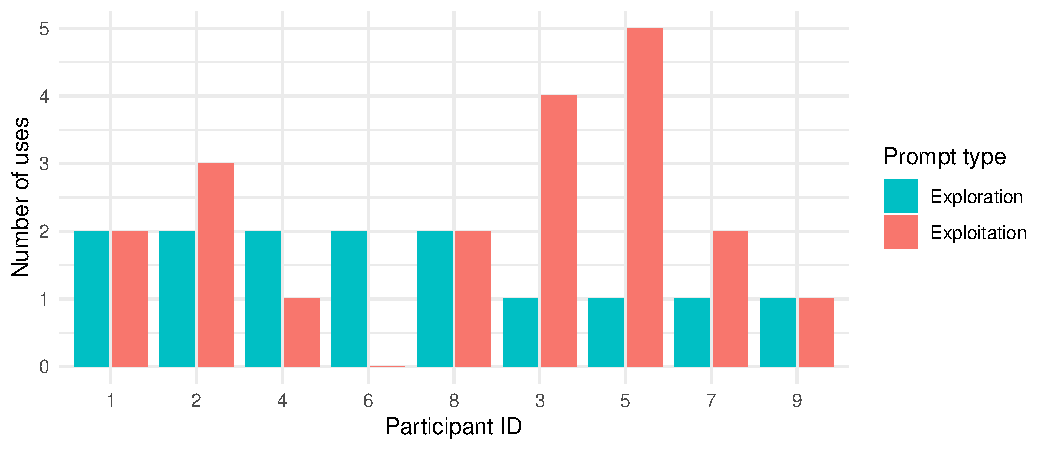
\includegraphics[width=1\linewidth]{XivxXp.pdf}
    \caption{Overall use of prompts, divided by type and ordered by the use of exploration prompts}
    \label{fig:XiXr}
\end{figure}


The results show that the total count of exploitation prompts is higher than exploration prompts (Table \ref{tab:Xi vs Xr}) and only two participants utilized more exploration than exploitation prompts (Figure \ref{fig:XiXr}). Participants employed a maximum of two explorations prompts, split almost equally between those that only explored one initial scenario, and those that explored an extra one (Figure \ref{fig:XiXr}). 
In contrast, there is more variability in the use of exploitation prompts.  Almost every participant –except from one– executed at least one exploitation action. No participant stopped at the minimum possible number of actions---generating and selecting an scenario without further prompting (Figure \ref{fig:XiXr}).  Despite a suggestive greater use of exploitation prompts between participants that only explored once (M = 3.0, SD = 1.8) instead of twice (M= 1.6 , SD = 1.4), there was no significant difference (Mann-Whitney $U$ = 14.5, \textit{p} = .89). Lastly, Table \ref{tab:chosenvsnonchosen} shows that the use of exploitation prompts is more frequent in the selected scenarios, instead of the discarded ones.



\subsubsection*{Use of Keywords}
% From here on is a copy paste from the relevant parts in .Rmd document - needs polishing and academic clarity
Overall, participants predominantly used the pre-defined guide's keywords over those from GPT (Table \ref{tab:Xi vs Xr}). Separating by prompt type, exploration prompts exclusively incorporated guide's keywords, whereas exploitation prompts mainly employed GPT's keywords, identified within the generated scenarios (Table \ref{tab:Xi vs Xr}). Individually, results show that 7 out of 8 participants that used exploitation prompts used at least one GPT's keyword with them.
Lastly, Table \ref{tab:chosenvsnonchosen} shows a predominant presence of GPT's keywords within the selected scenarios, contrary to the discarded ones. 


\subsubsection*{Selection of keywords and reported interests}

Regarding the use of the guide's set of keywords, Figure \ref{fig:KW of interest} shows that, overall, most of the guide's keywords used by participants corresponded to other's keywords---i.e., not initially provided by the participant in their first assignment. Regardless, we also observe that most participants, except for two, included at least one of their own keywords in their prompts. All in all, although inspired by the idea from  \textcite{niemi_artificial_2023} of using a socially-shared environment to allow users to explore their own representation, our study sessions did not support rich enough interactions to provide strong data on this question.

Overall, participants' used a wide range of concepts. Still, we found nine keywords that were used across three, or more, participants. These keywords were: university (n of participants = 6), benefit (n = 7 ), students (n = 4), ChatGPT 4 (n = 3), machine learning (n = 3), open ended problems (n = 3), and PhD researchers (n = 3). Unexpectedly, one of the GPT's keyword used by a participant matched with one of his own interests, therefore matching his personal interests.
\begin{figure}[H]
    \centering
    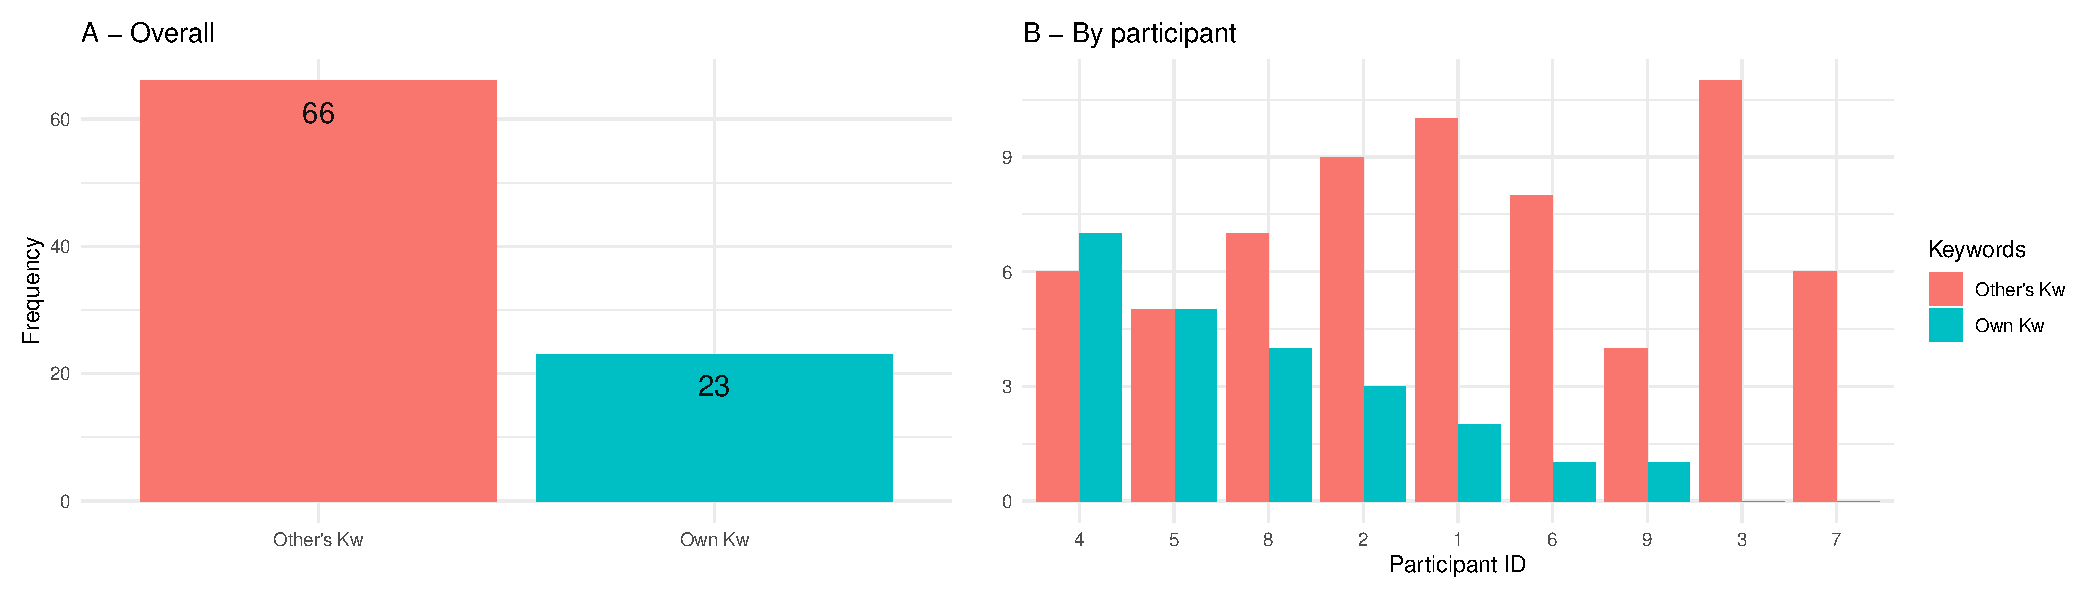
\includegraphics[width=1\linewidth]{KWofinterest.pdf}
    \caption{Participants utilization of Guide's keywords, separated in two categories: "Own Kw", personally contributed to the guide, and "Other's Kw", those contributed by their peers.}
    \label{fig:KW of interest}
\end{figure}


\subsection*{RQ 2 - Associations with Computational Thinking}

\subsubsection*{Estimated network structure}


Figure \ref{fig:Network A}  shows the relations between behavioral variables and CTS's scores.  The network was made up of 10 nodes, mean edge weight was 0.12, and 10 out of 36 possible connections were observed, consisting of 27\% of all possible connections. Figure \ref{fig:WeightAccA} shows the estimated edge weight stability. Only two statistical relationships show outside zero CIs: the use of exploration prompts and guide's keywords (tau = 0.77, p = .013) , and the use of exploitation prompts and GPT's keywords (tau = 0.74, p = .01).

CTS score divides the network in two clusters of nodes. One cluster is associated with the exploration prompts while the other is related to exploitation. 

Figure \ref{fig:Network B} expands on the relations between behavioral variables and the CTS's sub-factors. This network was made up of 13 nodes, mean edge weight was 0.089, and 24 out of 78 possible connections were observed consisting of 30.8\% of all possible connections. Figure \ref{fig:weightaccB} shows estimated edge weight stability for the expanded network. There are three new edges with CIs above zero: the amount of viewed keyword cards negatively relates both to creativity (tau = -0.76, p = .014) and algorithmic thinking (tau= -0.76, p = .014) CTS's scores, and the use of own keywords is negatively correlated with creativity CTS's scores (tau = -0.65, p = .022).  

\begin{figure}
    \centering
    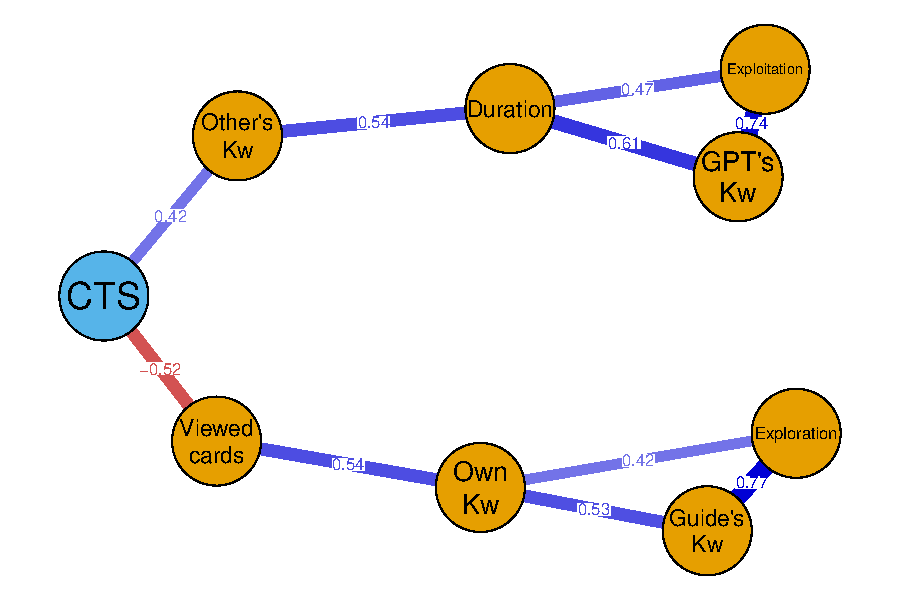
\includegraphics[width=0.75\linewidth]{NetworkA-nolegend.pdf}
    \caption{Estimated network structure between behavioral variables and CTS's scores. Nodes symbolize variables: Yellow for Interaction Behaviors, Blue for Computational Thinking Survey (CTS). Edges represent Kendall's tau correlations: Blue for positive, Red for negative. Spurious edges are filtered based on strength and significance, with thresholds set at $\tau > 0.4$, $p < 0.05$. }
    \label{fig:Network A}
\end{figure}
\begin{figure}
    \centering
    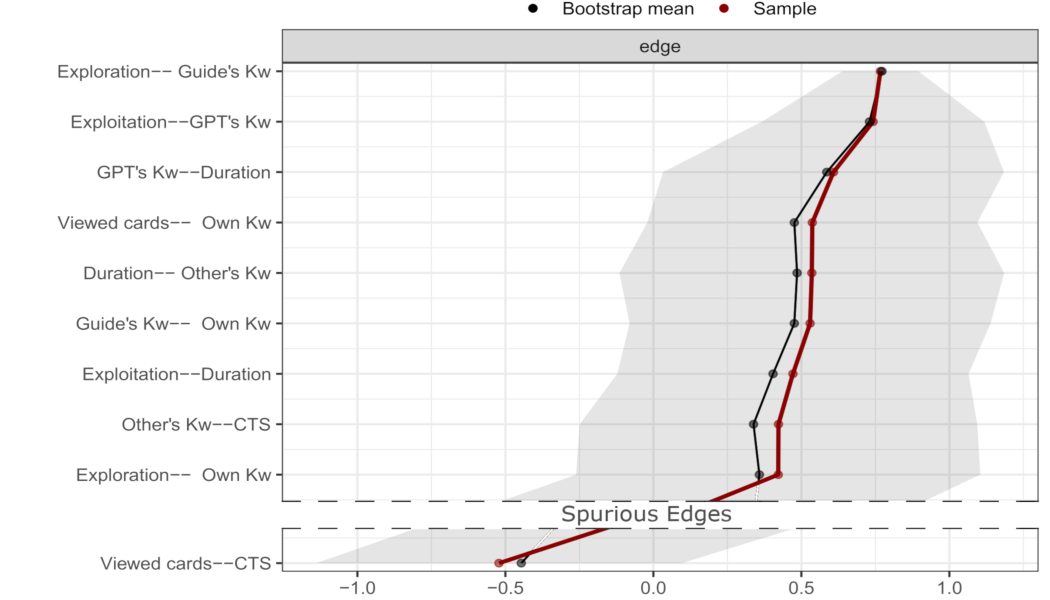
\includegraphics[width=0.75\linewidth]{EdgewgtsAcuttedscaled.pdf}
    \caption{Estimated edge weights' accuracy for network in Figure \ref{fig:Network A}. Estimated edge weights (red) compared to bootstrapped estimates (black) and their CIs (gray area), defined as 2-standard deviations. Spurious edges removed ($tau > 0.4$ and $p > 0.05$).}
    \label{fig:WeightAccA}
\end{figure}


%Expanded  - put the expanded one here

\begin{figure}
    \centering
    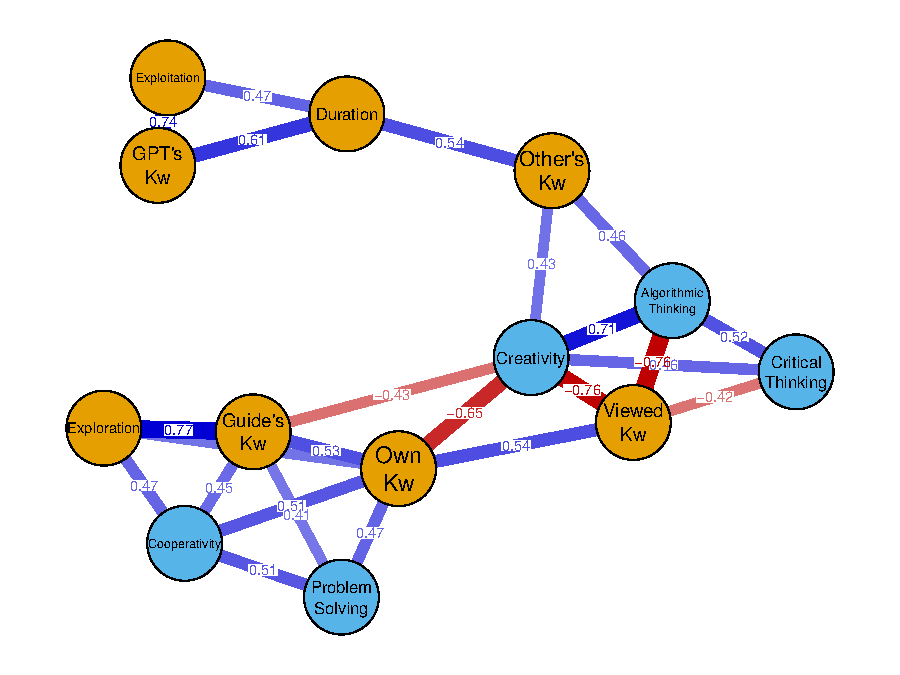
\includegraphics[width=1\linewidth]{NetworkB-nolegend.pdf}
    \caption{Estimated network structure between the behavioral variables and the CTS sub-factors' scores. Nodes symbolize variables: Yellow for Interaction Behaviors, Blue for Computational Thinking Survey's (CTS) sub-factors. Edges represent Kendall's tau correlations: Blue for positive, Red for negative. Spurious edges are filtered based on strength and significance, with thresholds set at $\tau > 0.4$, $p < 0.05$. }
    \label{fig:Network B}
\end{figure}

\begin{figure}
    \centering
    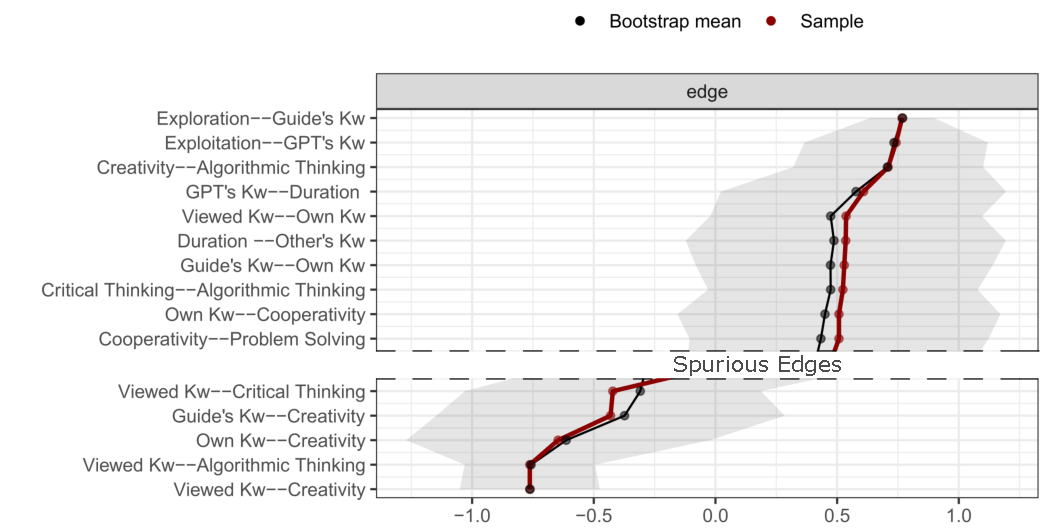
\includegraphics[width=0.75\linewidth]{EdgewgtsBcutted.pdf}
    \caption{Estimated edge weights' accuracy for network in Figure \ref{fig:Network B}. Estimated edge weights (red) compared to bootstrapped estimates (black) and their CIs (gray area), defined as 2-standard deviations. Spurious edges removed ($tau > 0.4$ and $p > 0.05$).}
    \label{fig:weightaccB}
\end{figure}



\section{Discussion}\label{Discussion}

We examine how do doctoral researchers display information foraging and computational thinking when using ChatGPT for a pedagogical design task. Considering the small and non-representative nature of our sample, we focus our study on describing our localized experience and generating hypothesis rather than generalizing findings for broader populations.  In the following section, we will discuss interesting findings in our two research questions, the limitations and further lines research.

\subsection*{RQ 1 - Foraging in AI generated landscapes}

Our study of students' interactions with GPT-4 in creating personalized case scenarios offers fresh insight to the application of Information Foraging Theory (IFT) in the context of AI-generated information landscapes. IFT has been useful in modeling users' goals and behaviors in web navigation \parencite{pirolli_rational_2005, pirolli_information_2007}, particularly emphasizing the roles of \textit{information scent} \parencite{spool1998web, pirolli_effects_2003,chi_scent_2000} and \textit{social cues} \parencite{sundar_news_2007, held_using_2010, muralidharan_social_2012} in driving users' foraging decision-making. Information scent can be briefly described as the subjective value of seen information in respect to the agent's inner goals \parencite{spool1998web, pirolli_computational_1997}. In digital environments, some interesting sources of valuable information scents are rankings, recommendations, forums, and other social cues that promote a shared sensemaking of information in different tasks and domains \parencite{fisher_distributed_2012, kittur_standing_2014}. These sources have been useful in driving web design, as they leverage users' existing knowledge and enhance efficiency in foraging tasks; they also help to understand the possible ways technology affects sensemaking \parencite{russell_cost_1993, kittur_costs_2013, pirolli_information_1999, chi_using_2001}.

The more dynamic nature of generative AI's information environments presents a novel paradigm for IFT analysis. Unlike the web, where information structures are mostly predefined and foraging paths are generally driven by links and query searches, AI-generated landscapes are primarily driven by prompting---a process fundamentally different from traditional web navigation. Due to its lack of structured informational landscapes, the decision-making processes in prompt construction, which drive both exploration and exploitation, deviates markedly from conventional web navigation. This may herald a paradigm shift in how users engage with information systems, underscoring the proactive and creative nature of information foraging in human-LLM interactions. This shift has profound implications for our understanding of IFT and its application in modern digital environments. 

In our study, participants' information foraging was driven by information scents identified both in the interaction design and in the AI-generated text. The structured interaction design, comprising the prompt templates and the set of keywords, served as a novel framework for examining how individuals navigate through AI-generated information landscapes, specifically in the context of human-LLM interactions. This design allowed an exploration of how participants navigate AI-generated informational landscapes through the construction of prompts that guide the generative process. We did not find a negative correlation between \textit{exploration} and \textit{exploitation} prompts, and they were mostly used in balance across participants (see Figure \ref{fig:XiXr}). Due to the lack of similar studies it is unclear whether these results represent high or a low number of prompt usage. Nevertheless, we found clear differences between the construction of these two distinct prompt types, primarily due to the distinct sources of the keywords employed and their relationship to participants' expressed interests.

\subsubsection*{Exploration prompts}

\textit{Exploration} prompt types, as defined in our study, were exclusively constructed using the guide's set of keywords, which were derived from the participants' provided keywords. By design, the first explored scenario must be driven by these keywords, as participants had no alternative sources. Intriguingly, we found that subsequent exploration prompts continued to be uniquely driven by these keywords (Table \ref{tab:Xi vs Xr}) . As we did not observed the use of GPT's keywords in exploration prompts, this suggest that participants' attention was focused on the content of the guide's set of keywords while constructing their exploration prompts, and followed the information scent sourced from their subjective interest therein. 

The prompt construction process provided interesting insights into participants' exploration efforts, particularly in their choice of keywords. Notably, participants frequently opted to include keywords contributed by others' (Figure \ref{fig:KW of interest}). This suggests a deviation from one probable pattern, where participants own keywords would be a main driver in their foraging behavior. Instead, we observed a predominant inclination towards of a shared and collaboratively built conceptual space, collected by the set of keywords. This finding suggests a meaningful social process, where participants' exploration efforts were influenced by a collective conceptual space rather than being driven solely by personal interests.  
Additionally, our analysis revealed trends in keyword selection. For example, certain keywords like 'university', were used by multiple participants (prompted by 6, for instance). By identifying these trends, we might raise insights about convergent or divergent class interests in specific topics. Such insights are valuable for pedagogical strategies and adaptations They can support the tailoring of course content, the implementation of student-centered teaching approaches, and the facilitation of organizing group discussions around common interest. Additionally, incorporating features aimed to collect and analyze the conceptual elements of prompts could reveal useful information for both shared sensemaking analysis and the refinement of pedagogical practices in educational settings that incorporate LLM-based systems.

Considering these findings, it becomes clear that special attention to interaction design elements, either in digital interfaces or hybrid activities, can compensate for the lack of static, pre-defined, and structured information, when analyzing foraging tasks in AI-informational landscape.
As ChatGPT interface does not offer visual information that can provide strong information scents to follow, the scent followed by participants to explore new information landscapes may emerge from the subjective value they assign to the design elements (i.e., prompt templates and set of keywords).

These design elements might be socially constructed, as our guide's keywords, and participants might explore and navigate AI-generated information landscapes through a collective conceptual space instead of merely following their individual interests and mental schemas. This suggests a meaningful role for the interface design and the contextual settings in guiding participants' initial foraging steps, especially during their first exploratory interactions. Consequently, digital studies and designs that facilitate human-LLM interaction might play a crucial role in either promoting or limiting these social aspects of prompt construction and users' behavior, depending on their design aims.

This finding could provide a direction for the development of human-LLM interaction designs in educational settings. Prior IFT research on the impact of social tags in web navigation \parencite{held_learning_2012, held_using_2010},  social annotation in web searches \parencite{fisher_distributed_2012}, and tagging systems \parencite{cress_collective_2013} demonstrates how social cues in web design can effectively enhance users foraging performance and promote a shared sense-making. In an interesting contribution, Kittur et al.´s \parencite*{kittur_standing_2014} study on the influence of social cues in web navigation illustrates how digital designs that capturing and aggregating mental schemas appealing to others can significantly enhance learning processes. Their research revealed that, when social cues are present, users would converge faster on the relevant dimensions of a task, effectively leveraging other users' mental schemas by enabling them to follow information scent trails explored by previous users. 

Following these contributions, Human-LLM interaction designs, especially in pedagogical settings, might substantially enhance learning processes by incorporating social cues in prompts construction. In the context of AI-generated information, where fixed and structured landscapes are absent, these social cues could include popular elements like frequently used concepts (keywords), common verb types and sentence structures (prompt templates), prompt ratings, records of positive/negative previous outcomes, and any other elements that may be unique to the prompting process. Such design elements might foster a constructivist and shared sense-making of learning goals, while also offering relevant insights into students' interests, focuses, and performance in human-LLM foraging tasks.

We emphasize the significance of this finding in contrast to a prevailing AIEd trend that advocates the potential of AI in individualized learning. A major trend identified by Holmes \& Tuomi in their literature review on AIEd \parencite*{holmes_state_2022} focuses on the potential of Intelligent Tutoring Systems' (ITS) to enhance personalized learning by identifying learners' individual interests and competencies, and creating tailored learning paths. The global pursuit of personalized learning has spurred the development of tools, methods, and curriculum through digital technologies \parencite{brunila_precision_2023}, yet its pedagogical definition remains ambiguous \parencite{holmes_technology-enhanced_2018, biesta_why_2010}. 
Critically, although numerous AIEd tools aim to profile students and curate individualized content, they often disconnect from educational theory, showing result-oriented approaches and therefore overlooking the complexities of education \parencite{holmes_state_2022, biesta_why_2010}. In our study, we diverge from this trend by allowing students to tailor their case scenarios, leading to a notable interplay between individual and peer interests. This approach contrasts with an ITS-informed strategy of simply tailoring personalized case scenarios based on their reported interests. Our observations highlight the influence of social elements in educational settings, often overlooked by the ITS's individual-centric focus. Further studies contrasting socialized and individualized strategies for LLM-based designs could provide valuable insights for AIEd future development, particularly in personalized learning.

Social elements may play a crucial role in early stages of information foraging tasks with ChatGPT, influencing decision-making during initial exploration prompts. In these early stages, it is vital for designers, educators and user interfaces to actively guide users, maximizing the value of these social elements. As the interaction progresses, however, the focus might shift from the design inputs to the AI-generated informational landscapes, suggested by the observed construction of exploitation prompts.  

\subsubsection*{Exploitation prompts}

Exploitation prompts were slightly more frequent that Exploration ones, a notable observation given their optional use, in contrast to the mandatory exploitation prompts required to start each interaction. Their importance becomes more pronounced when examining the scenarios: exploitation prompts appeared in all but one of the selected scenarios, with the majority (18 out of 20) used therein, as highlighter in Table \ref{tab:chosenvsnonchosen}. This trend suggests that exploiting the scenarios possibly added value to them, influencing the decision-making process in task completion and scenario selection. This suggestion aligns with the IFT definitions, where exploitation is viewed as a means to utilize and enrich an informational landscape to its fullest \parencite{cohen_should_2007, hills_exploration_2015}. This observation paves the way for future AI-based information foraging studies, offering potential to extend IFT into new domains and empirical data sources.

Regarding the keywords used in exploitation prompts, we found that they were derived either from our guide's set of keywords or from the GPT-generated information landscapes. Notably, there was a clear preference for using keywords sourced from GPT, as evidenced in Table \ref{tab:Xi vs Xr}. This preference suggests that, as the interaction progressed into the exploitation prompts, participants relied more on the AI-generated information landscapes for scents to follow, diverging from the guide's keywords conceptual guidance. It's important to note, however, that this shift towards AI-generated content still occurred within the context established by the initial exploration prompt. GPT's keywords, which were specific and contextualized to the AI-generated landscape, helped refine and specify elements within the generated scenario. Interestingly, one GPT keyword matched a participants' personal interest, underscoring the adaptability of GPT in tailoring content to user preferences. This observation aligns with the theoretically proposed capabilities of LLMs in adaptive learning, as proposed in the literature \parencite{bommasani_opportunities_2022, montenegro-rueda_impact_2023,  abu_talib_analytical_2021, lo_what_2023}. By generating specific, valuable information scents for the users to follow and exploit information landscapes, GPT might hold potential in enhancing users' foraging tasks.

While the use GPT's keywords facilitates context-specific exploitation of the information landscape, employing the guide's keywords serves a different purpose. These guide's keywords were useful to shift the focus towards concepts not included in the generated scenario. For instance, when ChatGPT omitted certain prompted keywords, guide's keywords in exploitation prompts helped prioritize specific elements or introduce new conceptual ideas. 

The predominance of GPT's keywords in exploiting AI-generated information landscapes introduces significant risks, namely hallucinations and overreliance, that are central to research and mitigate in foraging tasks. Hallucinations occur when LLMs generate incorrect information, posing a challenge for tasks that require objective precision. Furthermore, overreliance involves users mistakenly accepting these hallucinations as a valid knowledge, or incorrectly rejecting accurate information, a major challenge in safe AI integration \parencite{bubeck_sparks_2023, maynez_faithfulness_2020}. Unlike guide's keywords, whose relevancy could be reviewed during the design process, the AI-generated information necessitates real-time consideration by users. In educational settings, where users' expertise is developing, identifying LLMs' hallucinations might be particularly challenging. Subhash's \parencite*{subhash_can_2023} roughly showed that LLMs can have a strong persuasive influence over users preferences. Thus, recurrent reliance on GPT's keywords might, unknowingly, lead users down a rabbit-hole of misinformation. While in our AI-generated scenarios, which were speculative and hypothetical, this issue was mostly harmless and neglected, overreliance poses a substantial concern in tasks or subjects dealing with factual information. Consequently, there is a urging need for design elements that mitigate these risks in information foraging tasks

The potential benefits of social cues in human-LLM interactions, as previously discussed, can extend to mitigate risks like overreliance on AI-generated information. Current evidence suggests that only human annotators are able to effectively identify AI's hallucinations \parencite{maynez_faithfulness_2020}, and incorporating humans in AIEd designs (i.e., human-in-the-loop) is recommended for a safer integration of AI systems \parencite{bommasani_opportunities_2022, cardona_artificial_2023}. In designs like ours, implementing social cues more broadly, including the exploitation prompts, could create feedback loops with human involvement. This approach not only fosters collective value assessment of information and shared sense-making processes but also mitigates risks of overreliance by exposing users to others' experiences, much like Kittur et al.'s design \parencite*{kittur_standing_2014}. Altogether, controlled experiments focusing on the influence of social cues and the use of LLMs' generated information scents in exploration and exploitation behaviors within human-LLM interactions might not only reveal their pedagogical implications, but also offer deeper insights into IFT under the new AI technological landscape.


\subsection*{RQ 2 - Computational Thinking and Human-LLM interaction}

Turning our attention to our second research questions, our network analysis results suggest a clear distinction between exploration and exploitation prompt usage. As previously noted, exploration prompts uniquely use guide's keywords, whereas exploitation prompts are more aligned with GPT's keywords. Our estimated network delineates two distinct node clusters: one for exploration and another for exploitation, with the participants' CTS score acting as an interesting separator (see Figures \ref{fig:Network A} \& \ref{fig:Network B}). Even though no direct relation was observed between the CTS score and specific prompt types or keyword usage, our findings suggest that CTS score indirectly favors the use of exploitation over exploration prompts.When expanding upon the CTS sub-factors, creativity and algorithmic thinking emerge as key elements in differentiating these clusters, as evidenced in Figure \ref{fig:Network B}.
These factors show a negative correlation with the number of viewed keywords and a strong positive correlation with each other. Importantly, they present the only correlations between the behavioral and CTS data with CIs above zero (see Figure \ref{fig:weightaccB}). 
While other sub-factors are integrated into our estimated network, their less definitive CIs lead us to focus our discussion towards creativity and algorithmic thinking. Consequently, the subsequent sections will explore how creativity and algorithmic thinking potentially influence foraging behavior and prompt construction in human-LLM interactions.

\subsubsection*{Creativity}

In the context of IFT, the amount of viewed keywords indicates the volume of conceptual information available for prompt construction, chosen based on assessed subjective value, or information scent. This negative correlation between available information and their self-reported creativity suggests that participants with higher creativity scores may rely less on guide's keywords for prompt construction, and  their scenario co-creation task.

Participants with higher creativity scores, possibly more open to experimenting with new ideas, showed a tendency to use keywords different to their own ones. In contrast, those with lower creativity scores seemed to prefer the more structured guidance of our design, viewing more keywords and gravitating towards the ones aligned with their interests, as suggested by our network analysis.  

While creativity is often seen as a fuzzy and ill-defined concept \parencite{mishra_rethinking_2012, henriksen_creativity_2018}, technological innovations have arguably enhanced and broadened the ways humans can imagine, act and express themselves \parencite{zhao_world_2012, iste_ct_2015}. Supporting this, Shakeri et al. \parencite*{shakeri_saga_2021}'s pilot study on collaborative creative writing found that GPT, when acting as a co-writer, relieved creative pressures for users. By leaning on AI-generated suggestions (i.e., GPT's keywords) to continue their stories, users engaged in an AI-assisted discovery process while retaining a sense of ownership over the story.

Building on these ideas, it seems that more creative users may pay less attention to the interaction designed elements, focusing instead on the novel conversational dynamics offered by ChatGPT. Conversely, less creative participants may rely more on the design-provided guidance. This hypothesis is partially supported by a positive correlation with the exploitation cluster, driven predominantly by GPT's keywords, and a negative correlation with the exploration cluster, dominated by guide's keywords (see Figure \ref{fig:Network B}). However, these connections are indirect and further larger-scale studies are necessary to test these hypotheses. 

Understanding these dynamics might be crucial to grasp how user behavior and creativity interact in novel technological environments and to comprehend LLMs' impact on information foraging behavior. 

\subsubsection*{Algorithmic Thinking}

Reflecting the trends observed for creativity, our results suggest that participants with higher scores in algorithmic thinking also required less available information from the guide's keywords in their foraging task, as well as showing an increased use of others' keywords \ref{fig:Network B}. 

Algorithmic thinking, the skill of understanding, applying, assessing, and producing algorithms \parencite{brown2015introduction}, is central to computational thinking.. It is a key skill for computer science professionals \parencite{wing_computational_2006, angeli_computational_2020, cansu_overview_2019} and is integral to human-computer interactions, especially given the functional nature of computers that typically require automated, sequential, iterative, and logical instructions.

In AI-based systems,  where machine learning methods rely on somewhat different principles, such as big data and probabilistic models, this definition may require adaptations \parencite{marcus_modeling_2019, tedre_ct_2021}. Nevertheless, prompting involves an abstraction and automation process where users iteratively design, modify, and test different prompts to achieve desired outcomes, resembling processes of algorithmic thinking \parencite{repenning_proomting_2023}. 

Building on these considerations, our findings might suggest that participants with higher algorithmic thinking scores required less guidance from the pre-defined design keywords to construct effective prompts. 
They may possess a better understanding of prompting as the primary mode of interaction with ChatGPT. 
As Repenning \& Grabowski \parencite*{repenning_proomting_2023} note, prompting often requires multiple iterations for optimal results (i.e., following the conversation, or exploiting). This process may also be guided by ChatGPT's conceptual suggestion, as seen also in the studies by Yilmaz \& Karaoglan \parencite*{yilmaz_effect_2023} and Shakeri et al. \parencite*{shakeri_saga_2021} where participants tended to off-load creative and mechanical efforts thanks to the support of GPT's suggestions (i.e., GPT's keywords). These observations are slightly supported by algorithmic thinking scores positive association with the exploitation cluster in our estimated network (see Figure \ref{fig:Network B}). In other words, participants with higher algorithmic thinking might place greater value on exploiting ongoing conversations, as opposed to exploring new scenarios, to refine their AI-generated content. Furthermore, they could more rapidly discern the specific and contextual value of GPT's keywords for crafting effective exploitation prompts.

However, like the creativity sub-factor, no direct associations with specific prompt types were observed and further larger scale studies are needed to enrich our findings.


\subsection*{Limitations and Further Lines of Research}\label{Limitations}

Our study's primary limitation is its small sample size, which limits our ability to identify subtle relationships and increasing the possibility that our findings might differ from other samples. This limitation particularly restrained our network analysis, confining it to the entirety of the interaction rather than allowing for a comparative analysis between scenarios chosen by participants and those they disregarded. Such comparative analysis could enrich our understanding of how participants discern and value different AI-generated information. However, the structured and guided nature of our interaction offers opportunities for digital implementation, allowing for scalable and adaptable use across different domains. This open avenues for replication studies in diverse settings an populations. 

A following limitation is our exclusive focus on quantitative data. This approach restricted our analysis to observable factors. For a deeper understanding in users' foraging behavior, mixed-methods approaches incorporating both quantitative and qualitative data are required. These methods would allow us to explore users' subjective information needs and the scent-detection processes underlying their decisions-making \parencite{pirolli_information_1999}. Incorporating qualitative methods such as interviews, focus groups or content analysis could reveal more insights into users' motivations, mental schemas, and perceptions, enriching our understanding of their foraging behavior. Due to its utility as a inductive method for theoretical construction, grounded theory approaches \parencite{strauss_grounded_1997} can be particularly useful for analyzing AI-generated information landscapes and users' artifacts (i.e., subsequent assignments), aiding in understanding the effects of similar novel LLM-based implementations in educational contexts. A deeper focus on algorithmic thinking and creativity in human-LLM interactions may be of special interest. Potential instruments include the Creativity Support Index \parencite{cherry_quantifying_2014} for measuring digital technologies' support in creative processes, and the Algorithmic Thinking Test for Adults \parencite{lafuente_martinez_assessing_2022} for a focused measuring of algorithmic thinking within computational thinking. 

A final limitation concerns the categorization of keywords. As noted in our interaction design, the keywords, representing the main conceptual elements in our prompts, were categorized into broadly defined, somewhat nebulous categories. This imprecise system constrained our analytical capabilities, particularly in systematically exploring the convergence of keywords by topics (i.e, which "Subjects" or "Actors" were of more interest). Future research would benefit from using well-defined, exclusive conceptual categories. Such approach would enable a more detailed analysis of topical convergence in users' prompting processes. 

\subsection*{Final Remarks}\label{Conclusion}

Our study underlines the importance of thoughtful design in deploying LLMs in educational settings. As these models continue to scale up, its relevant that education specialists focus their efforts in understanding how the LLMs' novel capabilities affect and interact with user's cognitive processes for a positive integration of such systems.

We exemplify a design that is accessible to education specialists without requiring advanced programming skills. This approach is instrumental in advancing the broader implementation of LLM-based systems in educational settings. Understanding user behavior in AI-generated environments is key to developing intuitive, efficient, and user-centric AI systems. Aligning prompt construction and analysis with human foraging behaviors models might significantly improve the user experience and the effectiveness of AI tools in educational settings

Furthermore, integrating social cues that collect and aggregate users' mental schemas, inspired by Kittur et al. \parencite*{kittur_standing_2014}, could enhance collaborative learning and shared sense-making within different knowledge domains. This socialized approach to learning and digital design presents opportunities to integrate educational theoretical frameworks like social-constructivism \parencite{valente_maker_2019}, scaffolding \parencite{suwastini_schemes_2021, ak_role_2016}, and the zone of proximal development \parencite{crook_computers_1991, mckenney_designing_2013}.
These theoretical integrations could bridge the gap between data-driven AIEd implementations and educational theory, a major challenge identified in current AIEd research \parencite{holmes_state_2022, zawacki-richter_systematic_2019}. 

In conclusion, as LLMs evolve and become more accessible for various professionals, their integration into education by pedagogical experts could reconcile technological innovations with global educational challenges, fostering a more nuanced understanding of AI's impact on learning and development.






\printbibliography
%% if required, the content of .bbl file can be included here once bbl is generated
%%\input sn-article.bbl


\end{document}
